
\chapter{Appendix}
\label{chap:appendix}

\section{Solar surface differential rotation}
\label{sec:solar_surface_differential_rotation}
%surface differential rotation
The differential rotation of the solar surface is visible from sunspot observations and was first discovered by \citet{Scheiner1630}. It is caused by transport of angular momentum away from the rotation axis due to the Sun's inner thermal convective circulation.

%rotation period
\citet{Bartels1934} set the average synodic solar rotation period to 27~days for the definition of his solar rotation number. The Bartels Rotation Number counts the solar rotations starting with 8~February 1832. Later, Carrington determined a more accurate average solar rotation period of 27.2753~days, which is valid for solar latitudes of \SI{+-16}{\degree}, where sunspots usually are found. He defined the Carrington Rotation Number based upon this period, starting with 9~November 1853.
% http://wso.stanford.edu/words/Coordinates.html
% sidereal: 25.38~d (of 609.12~h Sun Fact Sheet...), synodic: 27.2753~d (derived)

%best-fitting function
The Sun's sidereal differential angular velocity can be approximated by the function\footnote{NASA's Sun Fact Sheet: \urlfoot{http://nssdc.gsfc.nasa.gov/planetary/factsheet/sunfact.html}}:
\begin{align}
	\omega_\odot(\theta) = \omega_\text{eq} + B \sin^2(\theta) + C \sin^4(\theta)	\,,	\label{eq:omega_differential}
\end{align}
with the heliolatitude $\theta$, the equatorial angular velocity $\omega_\text{eq} = \SI{14.37}{\degree\per\day}$, and the coefficients $B = \SI{-2.33}{\degree\per\day}$ and $C = \SI{-1.56}{\degree\per\day}$. I plotted this function in \autoref{fig:differential_rotation}.
\begin{figure}[htb]
	\fcapside[\FBwidth]{
		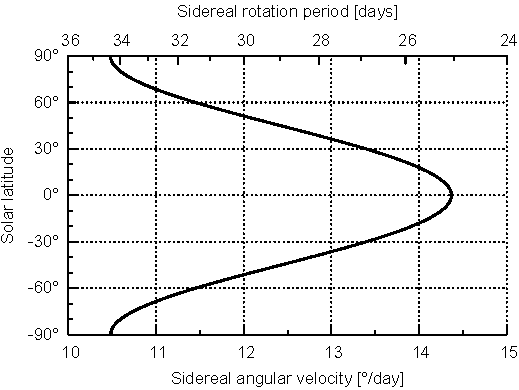
\includegraphics[width=0.6\textwidth]{figures_of_mine/gnuplots/differential_rotation.pdf}
	}{
		\caption{Diagram showing the angular velocity of the sidereal solar surface differential rotation over solar latitude. The upper x-axis shows the corresponding sidereal rotation period.}
		\label{fig:differential_rotation}
	}
	\addtocontents{lof}{\smallskip\protect\center I created the figure myself.\medskip}
\end{figure}
Thus, the solar equatorial sidereal rotation period is $T_\odot^\text{eq} = \SI{25.05}{\day}$ and the synodic period is
\begin{align}
	T_\odot^\text{eq,syn} &= \left(\frac{1}{T_\odot^\text{eq}} - \frac{1}{T_\text{E}}\right)^{-1}\\
	&= \SI{26.90}{\day}	\,,	\nonumber
\end{align}
with a Julian year as the Earth's orbital rotation period, $T_\text{E} = \SI{365.25}{\day}$.

The differential rotation differs locally in the different surface structures, such as sunspots and CHs. The angular velocity slows down with sunspot age and changes with how deep the structure is rooted in the interior \citep{Pulkkinen1998}. The average differential rotation profile is asymmetric in both hemispheres and also varies slightly with solar activity. Thus, \autoref{eq:omega_differential} is not a definite function, infact the average rotation rate is even slowing down over the last couple of solar cycles.

% Solar surface rotation period at equator\\
% sidereal: 25.05~d (Sun Fact Sheet...), synodic: 26.90~d (derived)\\
% Solar surface rotation period at poles:\\
% sidereal: 34.35~d (diff. rot. formula), synodic: 37.92~d (derived)\\
% are listed in \autoref{tab:solar_surface_rotation_periods}.\\
% \begin{table}[htb]\small
% 	\caption{Solar surface rotation periods for the equator, \SI{+-16}{\degree}~latitudes and the poles in sidereal and synodic rotation. accuracy to two digits...}
% 	\label{tab:solar_surface_rotation_periods}
% 	\centering
% 	\begin{tabular}{llll}
% 		\hline\hline
% 		\multirow{2}{*}{Rotation}	&Equator	&\SI{+-16}{\degree}~latitudes	&Poles\\
% 				&[d]	&\multicolumn{1}{c}{[d]}	&\multicolumn{1}{c}{[d]}\\
% 		\hline
% 		Sidereal	&25.05	&25.38	&34.35\\
% 		Synodic	&26.90	&27.2753$^\text{a}$	&37.92\\
% 		\hline
% 		\multicolumn{4}{l}{\footnotesize{$^\text{a}$Carrington solar rotation period}}
% 	\end{tabular}
% \end{table}


\section{Electric field at the magnetopause}
\label{sec:electric_field_at_the_magnetopause}
The Lorentz force law defines the electric and magnetic field vectors $\vect{E}$ and $\vect{B}$:
\begin{align}
	\vect{F} = q\,(\vect{E} + \vect{v} \times \vect{B})	\,.
\end{align}
It describes the force $\vect{F}$ that acts on a charge $q$ with velocity $v$. The full Ohm's law accounts for the Lorentz force:
\begin{align*}
	\vect{j} &= \sigma(\vect{E} + \vect{v} \times \vect{B})	& \Longleftrightarrow	&	&	\vect{E} &= - \vect{v} \times \vect{B} + \frac{\vect{j}}{\sigma}	\,.
\end{align*}
Solar wind is often approximated as an ideal MHD plasma having an infinite conductivity ($\sigma = \infty$). In this case electric fields do not generate electric currents ($\vect{j} / \sigma = 0$):
\begin{align}
	\vect{E} = - \vect{v} \times \vect{B}	\,.
\end{align}
Assuming a strict radial solar wind flow -- in x"~direction when using GSM coordinates ($v_\text{y} = v_\text{z} = 0$) -- the resulting electric field components become
\begin{align}
	\vect{E} =& \begin{bmatrix}
		0\\
		- v_\text{x} \cdot B_\text{z}\\
		v_\text{x} \cdot B_\text{y}
	\end{bmatrix}	\,.
\end{align}
Reconnection occurs only where the magnetic fields of the solar wind and magnetopause are antiparallel. Due to the magnetosphere's dipole topology, this is the case at the equator of the sunward magnetopause. If in addition the magnetospheric field is orientated along the z"~axis, the only remaining electric field component that contributes is
\begin{align}
	E_\text{y} = - v_\text{x} \cdot B_\text{z}	\,.
\end{align}

At the rest of the magnetopause surface facing the solar wind, the magnetospheric field deviates from the z"~direction, especially at higher latitudes. However, reconnection can occur there too if the solar wind magnetic field clock angle is oriented accordingly, see also \autoref{fig:Russell2007_fig4_10_VBbook_magnetopause_reconnection_regions_modified}. Thus, it makes sense to use the magnetic field's clock angle, which is defined as $\theta_c = \tan^{-1}\left(B_\text{y} / B_\text{z}\right)$, instead of just the field's $B_\text{z}$ component. The electric field becomes then
\begin{align}
	\vect{E} =& \begin{bmatrix}
		0\\
		- v_\text{x} \cdot |\vect{B_\text{yz}}| \, \cos(\theta_c)\\
		v_\text{x} \cdot |\vect{B_\text{yz}}| \cdot \sin(\theta_c)\\
	\end{bmatrix}	\,,
\end{align}
with $E_\text{y}$ containing the half-wave rectifier, see also \autoref{fig:coupling_angle_f}.


% Electromagnetism is one of the four fundamental forces at the common level of energy. In all situations examined in this thesis (solar wind plasma, magnetosphere) it is by far the strongest force and the others can be neglected.
% The Maxwell equations in differential notation:
% \begin{align}
% 	\text{div}\,\vect{B} &= 0\\
% 	\text{div}\,\vect{D} &= \rho\\
% 	\text{rot}\,\vect{H} &= \vect{j} + \dot{\vect{D}}\\
% 	\text{rot}\,\vect{E} &= - \dot{\vect{B}}
% \end{align}
% With the magnetic flux density $\vect{B}$ (aka magnetic field), the electric displacement field $\vect{D}$, the charge density $\rho$, the magnetic field $\vect{H}$, the electric field $\vect{E}$ and the current density $\vect{j}$.\\
% %note about B naming convention within this work as magnetic field strength


\section{Plasma beta}
\label{sec:plasma_beta}
The thermal pressure of a plasma is defined as $p = n k_\text{B} T$, with the number density $n$ and the Boltzmann constant $k_\text{B}$. However, according to magnetohydrodynamics (MHD), the magnetic energy density $w_\text{mag} = B^2 / (2 \mu_0)$, with the magnetic field strength $B$ and the permeability constant $\mu_0$, behaves like an additional pressure that adds to the thermal pressure of a plasma \citep[p.~50]{Kivelson1995}. The ratio of the thermal pressure to the magnetic pressure determines the behavior of the plasma. If the thermal pressure dominates the magnetic pressure (warm plasma), the plasma movements transport the magnetic field, else the plasma movements are guided by the magnetic field lines (cold plasma). This ratio is called plasma beta:
\begin{align}
	\beta &= \frac{p}{p_\text{mag}}	\,,\\
	&= \frac{2 \mu_0 n k_\text{B} T}{B^2}	\,.	\nonumber
\end{align}
The plasma at the photosphere has typical beta values around~14 and that of the low corona around~0.2 \citep{Gary2001}. Further up, beta raises again and the region where it equals~1 is defined as the source surface for the solar wind \citep{Schatten1969}.	% source surface where beta equals 1 (Schatten1969), at 0.6~Rs\\
This surface is typically located at about \SIrange{1.2}{2.5}{\Rs} \citep{Gary2001}.
% low source surface at 1.2~Rs (Gary2001)\\
% typical value at about 2.5~Rs\\

The solar wind usually has plasma beta values higher than~1 -- the solar magnetic field is carried away into the heliosphere. Together with the solar rotation, this effect creates the spiral form of the interplanetary magnetic field (Parker spiral). Yet in some solar wind structures, such as magnetic clouds, $\beta \ll 1$ and thus the magnetic field can still contain the plasma. Indeed, a change in plasma beta is a good predictor for the location of magnetic flux ropes in CME structures \citep{Riley2013,Savani2013}.

% https://omniweb.gsfc.nasa.gov/ftpbrowser/bow_derivation.html
% Plasma beta = thermal energy density (= thermal pressure) /magnetic energy density
%     = D*Np*k*Tp*8pi/B**2
% Beta = [(4.16*10**-5 * Tp) + 5.34] * Np/B**2 (B in nT)


%dynamic pressure $p_\text{dyn} = \rho v^2$\\
%ram pressure??\\
%VB1998p104


\section{Alfvén velocity}
\label{sec:alfvén_velocity}
The incompressible wave mode within MHD plasmas, the shear Alfvén wave, consists of periodic disturbances in the magnetic field orthogonal to its direction \citep{Alfven1942}. Alfvén waves are prevalent in open coronal regions and therefore occur in fast solar wind \citep{Cranmer2005}. Their propagation velocity is an important parameter to characterize a plasma. In an ideal incompressible MHD plasma (viscosity $\mu = 0$ and electrical conductivity $\sigma = \infty$) the kinetic and magnetic energy density are of equal value \citep[p.~51]{Kivelson1995}: 
\begin{align*}
	w_\text{kin} &= w_\text{mag}	& \Longleftrightarrow	&	&	\frac{\rho v^2}{2} &= \frac{B^2}{2 \mu_0}	\,,
\end{align*}
with the permeability constant $\mu_0$ and the total mass density $\rho$ of the charged plasma particles. Thus, the Alfvén velocity can be calculated via
\begin{align}
	v_\text{A} = \frac{|B|}{\sqrt{\mu_0 \rho}}	\text{\,.}
\end{align}
The wave's phase velocity is $v_\text{ph} = v_\text{A} \cos(\theta)$, with $\theta$ as the angle between wave propagation direction and magnetic field line, that is, Alfvén waves travel along magnetic field lines. They consist of periodic disturbances in the magnetic field, the electric field, the plasma velocity, and the current density. Plasma density, pressure, and magnetic field magnitude are not affected by them.

Additionally, there exist two types of compressional wave modes within MHD plasmas, the fast-mode wave and the slow-mode wave. The phase speeds of the three MHD waves meet $v_\text{fast} \geq v_\text{A} \geq v_\text{slow}$ \citep[p.~52]{Kivelson1995}. Within solar wind at \SI{1}{\au}, the typical frequency of Alfvén waves is 1--4 per hour and their average velocity is $v_\text{A} = \SI{56.8}{\km\per\s}$ \citep{Veselovsky2010}.\\	% at 1~au in 1963--2007\\

Alfvén critical surface...\\
sonic critical surfaces...\\

sonic and Alfvénic critical point positions (see Sittler \& Guhathakurta (1999))\\
sonic point and slow solar wind origin (Sheeley et al. 1997)\\


%wolfram alpha:
%solve v = 0.001*B/sqrt(mu*rho), B=5.6*10^-9, rho=5.3*10^6*1.66*10^-27, mu=4*pi*10^-7

%v_A=53.3km/s for r=1au; B=5.6nT; N=5.3cm-3
%v_A=91.5km/s for r=0.3 au; B=37.9nT; N=82.2cm-3
%v_A=280.6km/s for r=0.04 au; B=930.6nT; N=5274cm-3

%slow wind: v_A=28.5km/s for r=1au; B=4.7nT; N=13.0cm-3
%fast wind: v_A=68.7km/s for r=1au; B=5.7nT; N=3.3cm-3

%$v_\text{A} = 53$~km/s for $B = 5.6$~nT and $\rho = 5.3$~cm$^{-3}$


\section{Sun-Earth distance and rotation axes tilt}
\label{sec:sun_earth_orbit_geometry}
All interactions between Sun and Earth are governed by the geometry of Earth's orbit and the orientations of both bodies' rotation axes. The Earth orbit defines the ecliptic plane which is a convenient reference base for a few coordinate systems, see appendix \autoref{sec:coordinate_systems}.

% \subsection*{Solar distance}
The Sun-Earth distance can be derived from the orbital parameters of Earth\footnote{NASA's Earth Fact Sheet: \urlfoot{http://nssdc.gsfc.nasa.gov/planetary/factsheet/earthfact.html}}, the semimajor axis $a = \SI{1}{\au}$ and the eccentricity $e = \num{0.0167}$. Hence, the perihelion and aphelion distances are:
\begin{align*}
	r_\text{p} &= a (1 - e)	&	&\text{and}	&	r_\text{a} &= a (1 + e)\\
		&= \SI{0.9833}{\au}	\,,	&	&	&	&= \SI{1.0167}{\au}	\,,
\end{align*}
%perihelion, point on solar orbit with minimum distance to Sun\\
%aphelion, point on solar orbit with maximum distance to Sun\\
The exact solar distance at a given point in time can be obtained from the JPL~HORIZONS online ephemeris system\footnote{NASA/JPL HORIZONS Web-Interface: \urlfoot{http://ssd.jpl.nasa.gov/horizons.cgi}}, hosted by the Solar System Dynamics group at NASA's Jet~Propulsion Laboratory (JPL). In the year 2017, the Earth's perihelion was on 5~January.
% HORIZONS Web-Interface
% http://ssd.jpl.nasa.gov/horizons.cgi
% Ephemeris Type:	VECTORS
% Target Body:		Earth [Geocenter] [399]
% Coordinate Origin:	Sun (body center) [500@10]
% Time Span:		Start=2017-01-01, Stop=2017-12-31, Step=1 d
% Table Settings:	CSV format=YES
% Display/Output:	download/save (plain text file)
%-> distance:	9.833098226363186E-01
%-> diff. to 1 au:	0.166901774
%-> change to day before:	4.4e-6	-> 0.1669018(44)
The cosine approximation
\begin{align}
	r_\text{E}(t) = 1 - 0.0167 \cdot \cos\left(2 \pi \left(t - 2017 - \frac{5}{365}\right)\right)\,,
\end{align}
with $t$ in years, suffices for the plot of the seasonal changes in Earth's solar distance presented in \autoref{fig:Sun_Earth_geometry}.
\begin{figure}[htb]
	\fcapside[\FBwidth]{
		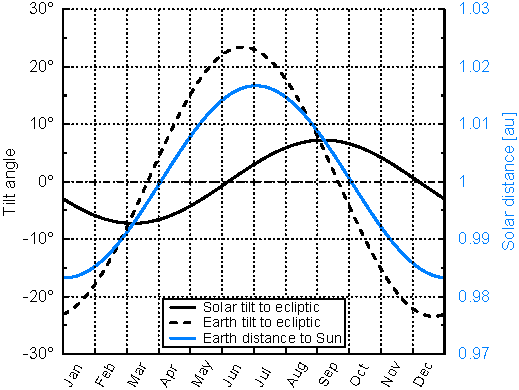
\includegraphics[width=0.6\textwidth]{figures_of_mine/gnuplots/Sun_Earth_geometry.pdf}
	}{
		\caption{Seasonal changes of the Sun's and the Earth's tilt angles to the ecliptic and of the Earth's solar distance. The curves are approximated with trigonometric fuctions.}
		\label{fig:Sun_Earth_geometry}
	}
	\addtocontents{lof}{\smallskip\protect\center I created the figure myself.\medskip}
\end{figure}
The total distance variation of \SI{3.34}{\%} has implications for the magnitude of the solar wind quantities measured at Earth, as most of them follow a power law distance dependency. Thus for example, the density varies about \SI{6.7}{\percent} between summer and winter because it scales with $r^{-2}$.

% perihelion/aphelion times:
%http://aa.usno.navy.mil/data/docs/EarthSeasons.php

% seasonal variation function:\\
% $x_\text{avg}(t) = a\,r_\text{E}(t)^b$\\
% values according to paper Venzmer2018, table 4:
% B_avg = 5.705(28)~nT\\
% B_med = 5.358(25)~nT\\
% n_avg = 6.845(47)~cm-3\\
% n_med = 5.424(33)~cm-3\\
% T_avg = 10.72(14)e5~K\\
% T_med = 6.357(64)e4~K\\
% v_avg = 4.47(11)e2~km/s\\
% v_med = 4.13(13)e2~km/s\\
% n_avg_p = 7.09 cm-3
% n_avg_a = 6.61 cm-3
% v_avg_p = 446.3 km/s
% v_avg_a = 447.7 km/s
% 
% % solar wind ram pressure (n*v^2) at perihelion:
% p_p = 1.41e18 m-1
% p_a = 1.32e18 m-1
% -> ram pressure varies by 6\% through the year\\


% \subsection*{Solar rotation axis tilt to the ecliptic}
The heliosphere is structured by the orientation of the solar rotation axis, e.g., the overall solar wind properties change with angular distance from the solar equator. The solar equator is inclined to the ecliptic by $i_\odot = \SI{7.25}{\degree}$\footnote{NASA's Sun Fact Sheet: \urlfoot{http://nssdc.gsfc.nasa.gov/planetary/factsheet/sunfact.html}}. Thus, viewed from Earth, the projected solar rotation axis tilt angle varies as the Earth is moving on its orbit. The seasonal change is plotted in \autoref{fig:Sun_Earth_geometry}, where the projected tilt at a given time is calculated by modulating $i_\odot$ with a sine, using the equation in \citet{Hapgood1992} and the time of vernal equinox. The projected tilt is zero at the equinoxes -- the vernal equinox in 2016 was on 20~March.
% vernal_equinox = 2016.0 + 2.0/12.0 + 20.0/366.0
% projected tilt from Earth: i_proj = i_sun * sin(beta)
% this years vernal equinox: eq = 2015.0 + 2.0/12.0 + 20.0/365.0 = 2015.2215
% actual separation angle from vernal equinox position: phi = (today - eq) * 360
% Ecliptic longitude of ascending node of the Sun's equator
% beta = phi - omega
% omega = 73.67 + 0.013\,958 * (today - 1850.0)
% tilt(x) = 7.25 * sin(-(73.67 + 0.013958 * (x - 1850.0)) + (-vernal_equinox + x) * 360.0)
% tilt(2016.0+(x-1.0)/12.0) with lines title "sine approx." ls 2 lw 2,\


% \subsection*{Earth rotation axis tilt to the ecliptic}
The orientation of the Earth's rotation axis to the Sun defines the solar wind flow angle onto the magnetosphere. The Earth's obliquity of the ecliptic is \SI{23.44}{\degree} and the resulting seasonal variation, seen in \autoref{fig:Sun_Earth_geometry}, influences the solar wind coupling efficiency with the magnetosphere and is reflected in geomagnetic activity as well.


\section{GSE, GSM, and HGI coordinate systems}
\label{sec:coordinate_systems}

A wise choice of coordinate system often eases the understanding and the calculation of a given problem, especially in geo- and astrophysics there exist an abundance of different coordinate systems. The coordinate systems used in this work are Earth- and Sun-centered and are described in the following. Three different Cartesian systems are applied: GSE, GSM, and HGI coordinates.

% GSE - Geocentric Solar Ecliptic
\subsection*{Geocentric Solar Ecliptic coordinates}
The Geocentric Solar Ecliptic (GSE) coordinates are centered at Earth and oriented with the ecliptic plane. The system's x"~axis points in direction of the Sun and its z"~axis in direction of the ecliptic north pole \citep{Russell1971,Hapgood1992}. The y"~axis completes the right-handed orthogonal system.
Thus compared to a fixed coordinate system, the GSE system completes one rotation around its z"~axis per year.
% Russell1971
% http://jsoc.stanford.edu/doc/keywords/Chris_Russel/Geophysical%20Coordinate%20Transformations.htm
% SPENVIS coordinate systems
% https://www.spenvis.oma.be/help/background/background.html

GSE coordinates are preferably used when looking at near-Earth solar wind measurements. In this work GSE coordinates are applied for the near-Earth solar wind measurements, e.g., with ACE data in Figures~\ref{fig:ACE_64s_v7_thesis_CIRs_2013-5-1_65_plot} and \ref{fig:ACE_64s_v7_thesis_CME_2013-6-26_6}.

% GSM - Geocentric Solar Magnetospheric
\subsection*{Geocentric Solar Magnetospheric coordinates}
The Geocentric Solar Magnetospheric (GSM) coordinates are also centered at Earth but oriented with its magnetic dipole axis. The x"~axis points in direction of the Sun and the z"~axis is parallel to the projection of the magnetic dipole axis on the plane normal to the x"~axis \citep{Russell1971,Hapgood1992}. Its direction is towards the negative magnetic pole located near the geographic North Pole. The dipole axis is defined by the centered geomagnetic dipole which is the best approximation to the International Geomagnetic Reference Field \citep{Thebault2015}. Again, the y"~axis completes the right-handed orthogonal system.
Relative to the GSE system, the GSM system shows a wobbling rotation around its x"~axis. The amplitude varies in time and is derived by the tilt of the Earth's rotation axis to the ecliptic normal (\SI{23.44}{\degree}) and the tilt of the dipole axis, which itself slightly changes over the years. Most of the last century, the tilt had an angle near \SI{11.5}{\degree} from the geographic poles, yet the current (2015) angular distance is \SI{9.53}{\degree} \citep{Thebault2015}.

GSM coordinates are useful in problems regarding the magnetosphere. These coordinates are applied throughout \autoref{chap:chapter2}.

% HGI - Heliographic Inertial
\subsection*{Heliographic Inertial coordinates}
The Heliographic Inertial (HGI) coordinates are centered at the Sun and oriented with its rotation axis. The z"~axis points northward parallel to the Sun's rotation axis. The x"~axis is parallel to the intersection line between the solar equatorial plane and the ecliptic plane \citep{Burlaga1984a}, which are inclined by \SI{7.25}{\degree}. This x"~axis points to the longitude of the ascending node which was at \SI{74.367}{\degree} on 1~January 1900 at 12:00~UT, but increases slowly with time (about \SI{1.4}{\degree} per century) due to the Earth's precession\footnote{Numbers according to NASA's COHOWeb documentation: \urlfoot{https://omniweb.gsfc.nasa.gov/coho/html/cw_data.html}}. The y"~axis completes the right-handed orthogonal system.
Over one year, the position of Earth oscillates within a HGI latitude range of \SI{+-7.25}{\degree}.

HGI coordinates are useful when looking at processes concerning the solar wind in the heliosphere. These coordinates are applied for the processing of the Helios data, e.g., in Figures~\ref{fig:Helios_r_b_ssn}, \ref{fig:Helios12_orbits_ecliptic_polar}, and \ref{fig:helios_data_frequency}.


\section{True skill statistic}
\label{sec:true_skill_statistic}
The true skill statistic (TSS) or true skill score is a means for measuring the predictive value of a variable. It was developed by \citet{Hanssen1965} for evaluating different predictors for rain and dry weather conditions. Therefore it is also often called the Hanssen-Kuipers skill score or the Hanssen-Kuipers discriminant. As with other skill scores, the TSS is based on a 2x2 contingency table that categorizes forecasted and observed events, see the \autoref{tab:contingency_table}.
\begin{table}[htb]
	\caption{Generic contingency table for categorizing forecasted and observed events. The designations for the event counts are given in parentheses.}
	\label{tab:contingency_table}
	\centering
	\begin{tabular}{ll|cc}
		\hline\hline
				&\multicolumn{3}{c}{\hspace*{1em}Observed}\\
				&	&Yes	&No\\
		\cline{2-4}
		\multirow{4}{*}{Forecasted}	&\multirow{2}{*}{Yes}	&Hit	&False alarm\\
				&	&($n_\text{H}$)	&($n_\text{FA}$)\\
				&\multirow{2}{*}{No}	&Miss	&Correct null\\
				&	&($n_\text{M}$)	&($n_\text{CN}$)\\
		\hline
	\end{tabular}
\end{table}
The following ratios, derived from this kind of table, reveal relevant information about the forecast quality \citep{Doswell1990}: The proportion of correct predictions
\begin{align}
	\mathit{PC} = \frac{n_\text{H} + n_\text{CN}}{n_\text{H} + n_\text{FA} + n_\text{M} + n_\text{CN}}	\,,
\end{align}
the probabilities of detection and of false detection (i.e., the hit rate and the false alarm rate)
\begin{align*}
	\mathit{POD} &= \frac{n_\text{H}}{n_\text{H} + n_\text{M}}	&	&\text{and}	&	\mathit{POFD} &= \frac{n_\text{FA}}{n_\text{FA} + n_\text{CN}}	\,,
	\intertext{as well as the false alarm and detection failure ratios}
	\mathit{FAR} &= \frac{n_\text{FA}}{n_\text{FA} + n_\text{H}}	&	&\text{and}	&	\mathit{DFR} &= \frac{n_\text{M}}{n_\text{M} + n_\text{CN}}	\,.
\end{align*}
The TSS is the difference between the hit rate and the false alarm rate\footnote{False alarm rate -- not to be confused with false alarm ratio.} and thus it is calculated as follows \citep[Eq.~15]{Hanssen1965}:
\begin{align}
	\mathit{TSS} &= \mathit{POD} - \mathit{POFD}\\
		&= \frac{n_\text{H} \cdot n_\text{CN} - n_\text{FA} \cdot n_\text{M}}{\left(n_\text{H}+n_\text{M}\right) (n_\text{FA}+n_\text{CN})}	\,.	\nonumber	\label{eq:true_skill_score}
\end{align}
Its value is in the range from -1 to 1, with 1 representing an ideal prediction, 0 a random prediction, and -1 an ideal negative prediction. The TSS is positive if the hit rate is higher than the false alarm rate.

In the case of rare event forecasting, the contingency table is dominated by correct nulls and the TSS approaches the hit rate. \citet{Doswell1990} show that the Heidke skill score is superior in these situations, in that it considers correct null forecasts in a controlled way. They recommend to use the Heidke skill score in preference to TSS for rare event forecasting. Other often applied skill scores are the threat score, also called critical success index or Gilbert score, and the equitable threat score. However, the TSS is commonly applied to evaluate and compare space weather prediction methods, especially in forecasting the \Kp~index \citep{Detman1999,Wing2005,Savani2017}. The TSS is used in the verification analysis of operational geomagnetic storm forecasts as well, for example at the SIDC\footnote{SIDC's Verification Analysis of the SIDC Forecast website: \urlfoot{http://sidc.be/forecastverification/K_index_storm_5+.php}}.


% Fraction Correct is given by [0,1]\\
% chance hits
% ch=((x+y)*(x+z))/(w+x+y+z)


\section{Lognormal distribution}
\label{sec:lognormal_distribution}
This is a small summary about the lognormal probability distribution. The lognormal distribution is the distribution of a random variable $X$ if the logarithm of $X$ conforms to a normal distribution \citep[p.~780]{Bronstein2000}. Its shape is highly asymmetric, however in a semi-log plot the Gaussian bell curve is recognizable, see \autoref{fig:lognormal_semi_log}.
\begin{figure}[htb]
	\begin{floatrow}
		\ffigbox{
			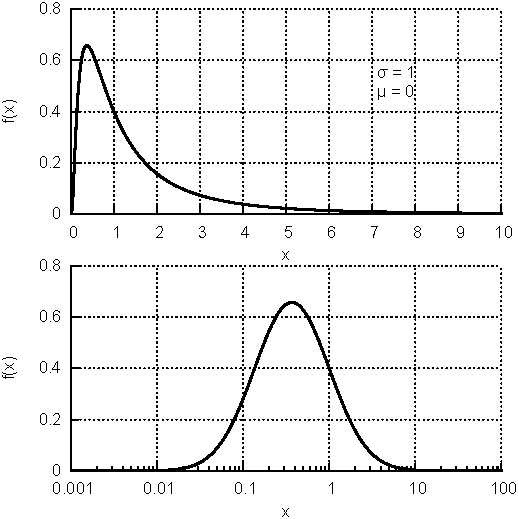
\includegraphics[width=0.46\textwidth]{figures_of_mine/gnuplots/lognormal_semi_log.pdf}
		}{
			\caption{Lognormal probability density function plotted in a linear (top panel) and semi-log (bottom panel) way. Both distributions have the parameters $\sigma = 1$ and $\mu = 0$.}
			\label{fig:lognormal_semi_log}
		}
		\addtocontents{lof}{\smallskip\protect\center I created the figure myself.\medskip}
		\ffigbox{
			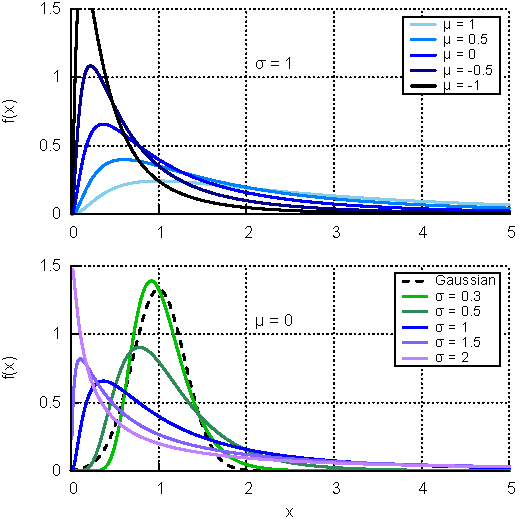
\includegraphics[width=0.46\textwidth]{figures_of_mine/gnuplots/lognormal_ms_b.pdf}
		}{
			\caption{Sets of five different lognormal distributions plotted with a fixed $\sigma$ (top panel) and a fixed $\mu$ (bottom panel). The Gaussian curve is drawn for comparison.}
			\label{fig:lognormal_ms_b}
		}
		\addtocontents{lof}{\smallskip\protect\center I created the figure myself.\medskip}
	\end{floatrow}
\end{figure}
Its probability density function is
\begin{align}
	f(x) &= \frac{1}{\sigma \sqrt{2 \pi} x} \, \text{e}^{- \frac{(\ln x - \mu)^2}{2 \sigma^2}}	\,,
\end{align}
with the location ($\mu$) and the shape parameter ($\sigma$). Changes in $\mu$ affect both the horizontal and vertical scaling of the function, whereas $\sigma$ has an influence on its shape, see the graphs with different $\mu$ and $\sigma$ in \autoref{fig:lognormal_ms_b}.

A lognormal distribution adheres to the general properties noted in the following. As it is a probability distribution, its area is normalized:
\begin{align*}
	\int_0^\infty f(x) \text{d} x = 1	\,.
\end{align*}
For a lognormally distributed random variable, the geometric moments mean, standard deviation, and variance are calculated from:
\begin{align*}
	&\mu_\text{g} = \text{e}^\mu	\,,	&	&\sigma_\text{g} = \text{e}^\sigma	\,,	&	&\text{var}_\text{g} = \text{e}^{\sigma^2}	\,.\\
	\intertext{Whereas its arithmetic moments are derived from:}
	&\mu_\text{a} = \text{e}^{\mu + \frac{\sigma^2}{2}}	\,,	&	&\sigma_\text{a} = \text{e}^{\mu + \frac{\sigma^2}{2}} \, \left(\text{e}^{\sigma^2} - 1\right)	\,,	&	&\text{var}_\text{a} = \sigma_\text{a}^2\,.
\end{align*}
Further useful characteristics are the positions of the median and the mode:
\begin{align*}
	&x_\text{median} = \text{e}^{\mu}	\,,\\
	&x_\text{mode} = \text{e}^{\mu - \sigma^2}	\,.
\end{align*}
Note that for the lognormal distribution its median is equal to its geometric mean. In the limit of $\sigma \ll 1$ the lognormal shape converges to a Gaussian, see the lower panel of \autoref{fig:lognormal_ms_b}.

Most distributions in nature deviate from the simple Gaussian shape and are to some extent skewed. Indeed, almost all natural quantities which can only be positive are lognormally distributed. Such distributions are found in all fields of sciences \citep{Limpert2001}, for example in biology (size and weight of individuals in populations; species abundance), in medicine (latency periods and survival times of diseases), in social sciences (age of marriage), in linguistics (lengths of words and sentences), in economics (household income), and in geophysics (distribution of mineral resources in the Earth's crust). Obviously measurements of certain solar wind quantities and geomagnetic indices conform to lognormal distributions as well.


\section{Astronomical constants}
\label{sec:astronomical_constants}

Astronomical unit: $\SI{1}{\au} = \SI{149597870.700}{\km}$ \citep{Luzum2011}\\
Nominal solar radius (photosphere): $R_\odot = \SI{695700}{\km}$ \citep{Mamajek2015}\\
% Nominal solar effective temperature (photosphere): $T_{\text{eff}\odot} = \SI{5772}{\kelvin}$ \citep{Mamajek2015}\\
Solar rotation axis tilt to ecliptic: $i_\odot = \SI{7.25}{\degree}$ (NASA's Sun Fact Sheet\footnote{NASA's Sun Fact Sheet website: \urlfoot{http://nssdc.gsfc.nasa.gov/planetary/factsheet/sunfact.html}})\\ %C3; Obliquity to ecliptic
Earth rotation axis tilt to ecliptic: $i_\text{E} = \SI{23.439279}{\degree}$ \citep{Luzum2011}\\ %C3; Obliquity to ecliptic

\noindent Notable online resources for astronomical constants:
\begin{itemize*}
	\item IAU 2009 values and best estimates, IAU Division I Working Group, Numerical Standards for Fundamental Astronomy \citet{Luzum2011}:\\
	\urltext{http://maia.usno.navy.mil/NSFA/}
	
	\item The Astronomical Almanac Online, \citet{USNAO2017}:\\
	\urltext{http://asa.usno.navy.mil/static/files/2016/Astronomical_Constants_2016.pdf}
	
	\item NASA's Planetary~Fact~Sheets:\\
	\urltext{https://nssdc.gsfc.nasa.gov/planetary/planetfact.html}
	
\end{itemize*}

% Solar mass: $M_\odot = \SI{1.9884(2)e30}{\kg}$ \citep{USNAO2017}\\
% Sun escape velocity: $v_\text{esc} = \SI{617.6}{\km\per\s}$ (Sun Fact Sheet...)\\
% Solar surface rotation period at equator, sidereal: 25.05~d (Sun Fact Sheet...)\\


\section{List of acronyms}
\label{sec:list_of_acronyms}

fit acronyms into one page!!\\

Generic acronyms:
\begin{description}[labelwidth=1.2cm]
	\item[ANN] artificial neural network
	\item[BDE] bidirectional electrons
	\item[DB] disparition brusques
	\item[Dst] disturbance storm time
	\item[CH] coronal hole
	\item[CIR] corotating interaction region
	\item[CME] coronal mass ejection
	\item[DQCS] dipole plus quadrupole plus current sheet
	\item[EUV] extreme ultraviolet
	\item[GNSS] global navigation satellite system
	\item[GSE] geocentric solar ecliptic
	\item[GSM] geocentric solar magnetospheric
	\item[HCS] heliospheric current sheet
	\item[HGI] Heliographic Inertial
	\item[HMF] heliospheric magnetic field
	\item[HPS] heliospheric plasma sheet
	\item[HSS] high speed stream
	\item[ICME] interplanetary coronal mass ejection
	\item[IMF] interplanetary magnetic field
	\item[Kp] planetare Kennziffer
	\item[MAD] mean absolute deviation
	\item[MBP] magnetic bright point
	\item[MC] magnetic cloud
	\item[MHD] magnetohydrodynamic
	\item[MVA] minimum variance analysis
	\item[SB] sector boundary
	\item[SAR] sum of absolute residuals
	\item[SEP] solar energetic particle
	\item[SIR] stream interaction region
	\item[SSN] sunspot number
	\item[TEC] total electron content
	\item[TSS] true skill statistic
\end{description}

\noindent Specific acronyms:
\begin{description*}
	\item[ACE] Advanced Composition Explorer
	\item[AFFECTS] Advanced Forecast For Ensuring Communications Through Space
	\item[AIA] Atmospheric Imaging Assembly
	\item[BSS] Bothmer-Schwenn scheme
	\item[CAT] CME Analysis Tool
	\item[CCMC] Community Coordinated Modeling Center
	\item[CDAWeb] Coordinated Data Analysis Web
	\item[CEDAR] Coupling, Energetics and Dynamics of Atmospheric Regions
	\item[CGAUSS] Coronagraphic German And US SolarProbePlus Survey
	\item[DDC] DoomsDayCalculator
	\item[DSCOVR] Deep Space Climate Observatory
	\item[EVE] EUV Variability Experiment
	\item[FP7] Framework Programme 7
	\item[GCS] Graduated Cylindrical Shell
	\item[GFZ] GeoForschungsZentrum
	\item[GSFC] Goddard Space Flight Center
	\item[HELCATS] Heliographic Cataloging, Analysis and Techniques Service
	\item[HMI] Helioseismic Magnetic Imager
	\item[IAG] Institute for Astrophysics Göttingen
	\item[IAGA] International Association of Geomagnetism and Aeronomy
	\item[ISGI] International Service of Geomagnetic Indices
	\item[LASCO] Large Angle and Spectrometric COronagraph
	\item[MAG] name of the Magnetometer on the ACE spacecraft
	\item[MDI] Michelson Doppler Imager
	\item[MMS] Magnetospheric Multiscale
	\item[NASA] National Aeronautics and Space Administration
	\item[NOAA] National Oceanic and Atmospheric Administration
	\item[OMNI] name of the multi-source data set
	\item[OPTIMAP] OPerational Tool for Ionospheric Mapping And Prediction
	\item[PSP] Parker Solar Probe
	\item[RTSW] Real Time Solar Wind
	\item[ROB] Royal Observatory of Belgium
	\item[SDO] Solar Dynamics Observatory
	\item[SIDC] Solar Influences Data Center
	\item[SPDF] Space Physics Data Facility
	\item[SOHO] Solar and Heliospheric Observatory
	\item[STEREO] Solar TErrestrial RElations Observatory
	\item[SWS] Solar Wind Structures
	\item[SWEPAM] Solar Wind Electron Proton Alpha Monitor
	\item[SWPC] Space Weather Prediction Center
	\item[UGOE] University of Göttingen
	\item[WDC-SILSO] World Data Center-Sunspot Index and Long-term Solar Observations
	\item[WISPR] Wide-field Imager for Solar Probe
\end{description*}

% find
% \n(.*) -- (.*)\\\\
% replace
% \n\t\\item[\1] \2

% 	\item[] 

